\documentclass{article}
\usepackage{pgfplots}
\pgfplotsset{compat=1.18}
\begin{document}
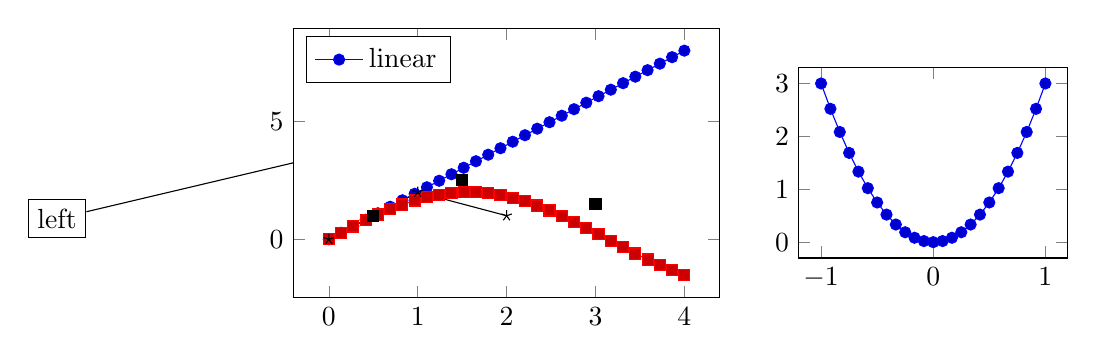
\begin{tikzpicture}
  \def\k{2}
  \node[draw] (left) at (-2,1) {left};
  \begin{axis}[name=main, at={(1cm,0cm)}, width=7cm, height=5cm, domain=0:4, samples=30, legend pos=north west]
    \addplot {\k*x};
    \addlegendentry{linear}
    \addplot+[smooth] {sin(deg(x))*\k};
    \addplot[only marks, mark=square*] table {
      x y
      0.5 1
      1.5 2.5
      3 1.5
    };
    \addplot coordinates {(0,0) (1,\k) (2,1)};
  \end{axis}
  \def\k{3}
  \begin{axis}[at={(main.east)}, anchor=west, xshift=1cm, width=5cm, height=4cm, domain=-1:1]
    \addplot {\k*x^2};
  \end{axis}
  \draw (left) -- (main.west);
\end{tikzpicture}
\end{document}
